% ===============================================================================
\section{Introduction}\label{sec:introduction}
\wingj is an open-source image processing toolkit for unsupervised, multi-scale quantification of biological systems (organ systems or body systems) \autocite{schaffter2013}. \wingj provides tools for automatic structure detection from confocal fluorescence images, which consists in generating a parametric model that accurately describes the morphology of an organ system (e.g. \droso wing pouch) or body system (e.g. \droso embryo). The approach we developed is based on the design of many \emph{detection modules} that each takes care of identifying a specific feature of the overall structure to model (\figref{fig:detection_modules_overview}). This includes the detection and modeling of fluorescence patterns including the detection of compartments, the identification of the trajectory of fluorescence boundaries, etc. A consistent parametric model of the overall structure to quantify is then generated by integrating the outputs of the different detection modules.\\

% \wingj is an open-source Java toolkit for systematic quantification of biological organisms or organs. \wingj provides tools to automate the segmentation of the morphological of the \textit{Drosophila melanogaster} wing pouch and \textit{Drosophila melanogaster} embryo from stacks of fluorescence confocal images.\\
% 
% The parametric structure model generated by \wingj allows to measure specific features such as boundary lengths, compartment areas and perimeters, etc. These measurements are then converted from pixel unit to physical units (e.g. \mum) using meta-information included by the microscopes in the input images. Once a structure model has been identified, additional tools implemented in \wingj can be used, for instance to quantify expression or count stained nuclei inside the space of the inferred structure.\\

% \wingj is an open-source Java toolkit for systematic quantification of biological organisms or organs. \wingj provides tools to automatically segment the morphological structure of the \textit{Drosophila melanogaster} wing pouch and embryo from stacks of fluorescence confocal images. The \textit{structure model} identified by \wingj has several applications. First, it is used to measure specific features of the structure such as boundary lengths or compartment perimeters and areas. Measurements are converted from pixel unit to physical units (e.g. \mum and \mumsquare) using meta-information included by the microscopes in the input images. Once a structure model has been inferred, additional tools available in \wingj enable the easy quantification of expression profiles and \textit{maps} inside the space of the structure model. Furthermore, we provide an automatic \textit{nuclei detection} method that, when combined with a structure model, returns the number of nuclei included in the system of interest (here the structure model is used to define a subspace inside the 3D image space).\\
% 
% In \wingj, the \textit{structure detection} refers to a sequence of \textit{detection modules} designed to identify specific features of the overall structure to model \citep{schaffter2013}. In the detection of the \textit{Drosophila} wing pouch structure for instance, one of the first module applied identifies where the anterior/posterior (A/P) and dorsal/ventral (D/V) boundaries intersect. Yet another module applies active contour algorithms (also called \textit{snakes}) to segment the four compartments DA, DP, VA, and VP that are included in the wing pouch. A parametric model of the structure is then generated by combining the different output of the detection modules. We developed and implemented as much as eight detection modules to identify the wing pouch structure \citep{schaffter2013}, whose respective output is shown in Figure~\ref{fig:wingj_wpouch_detection_modules_intro}.\\

\begin{figure}[!h]
\centering
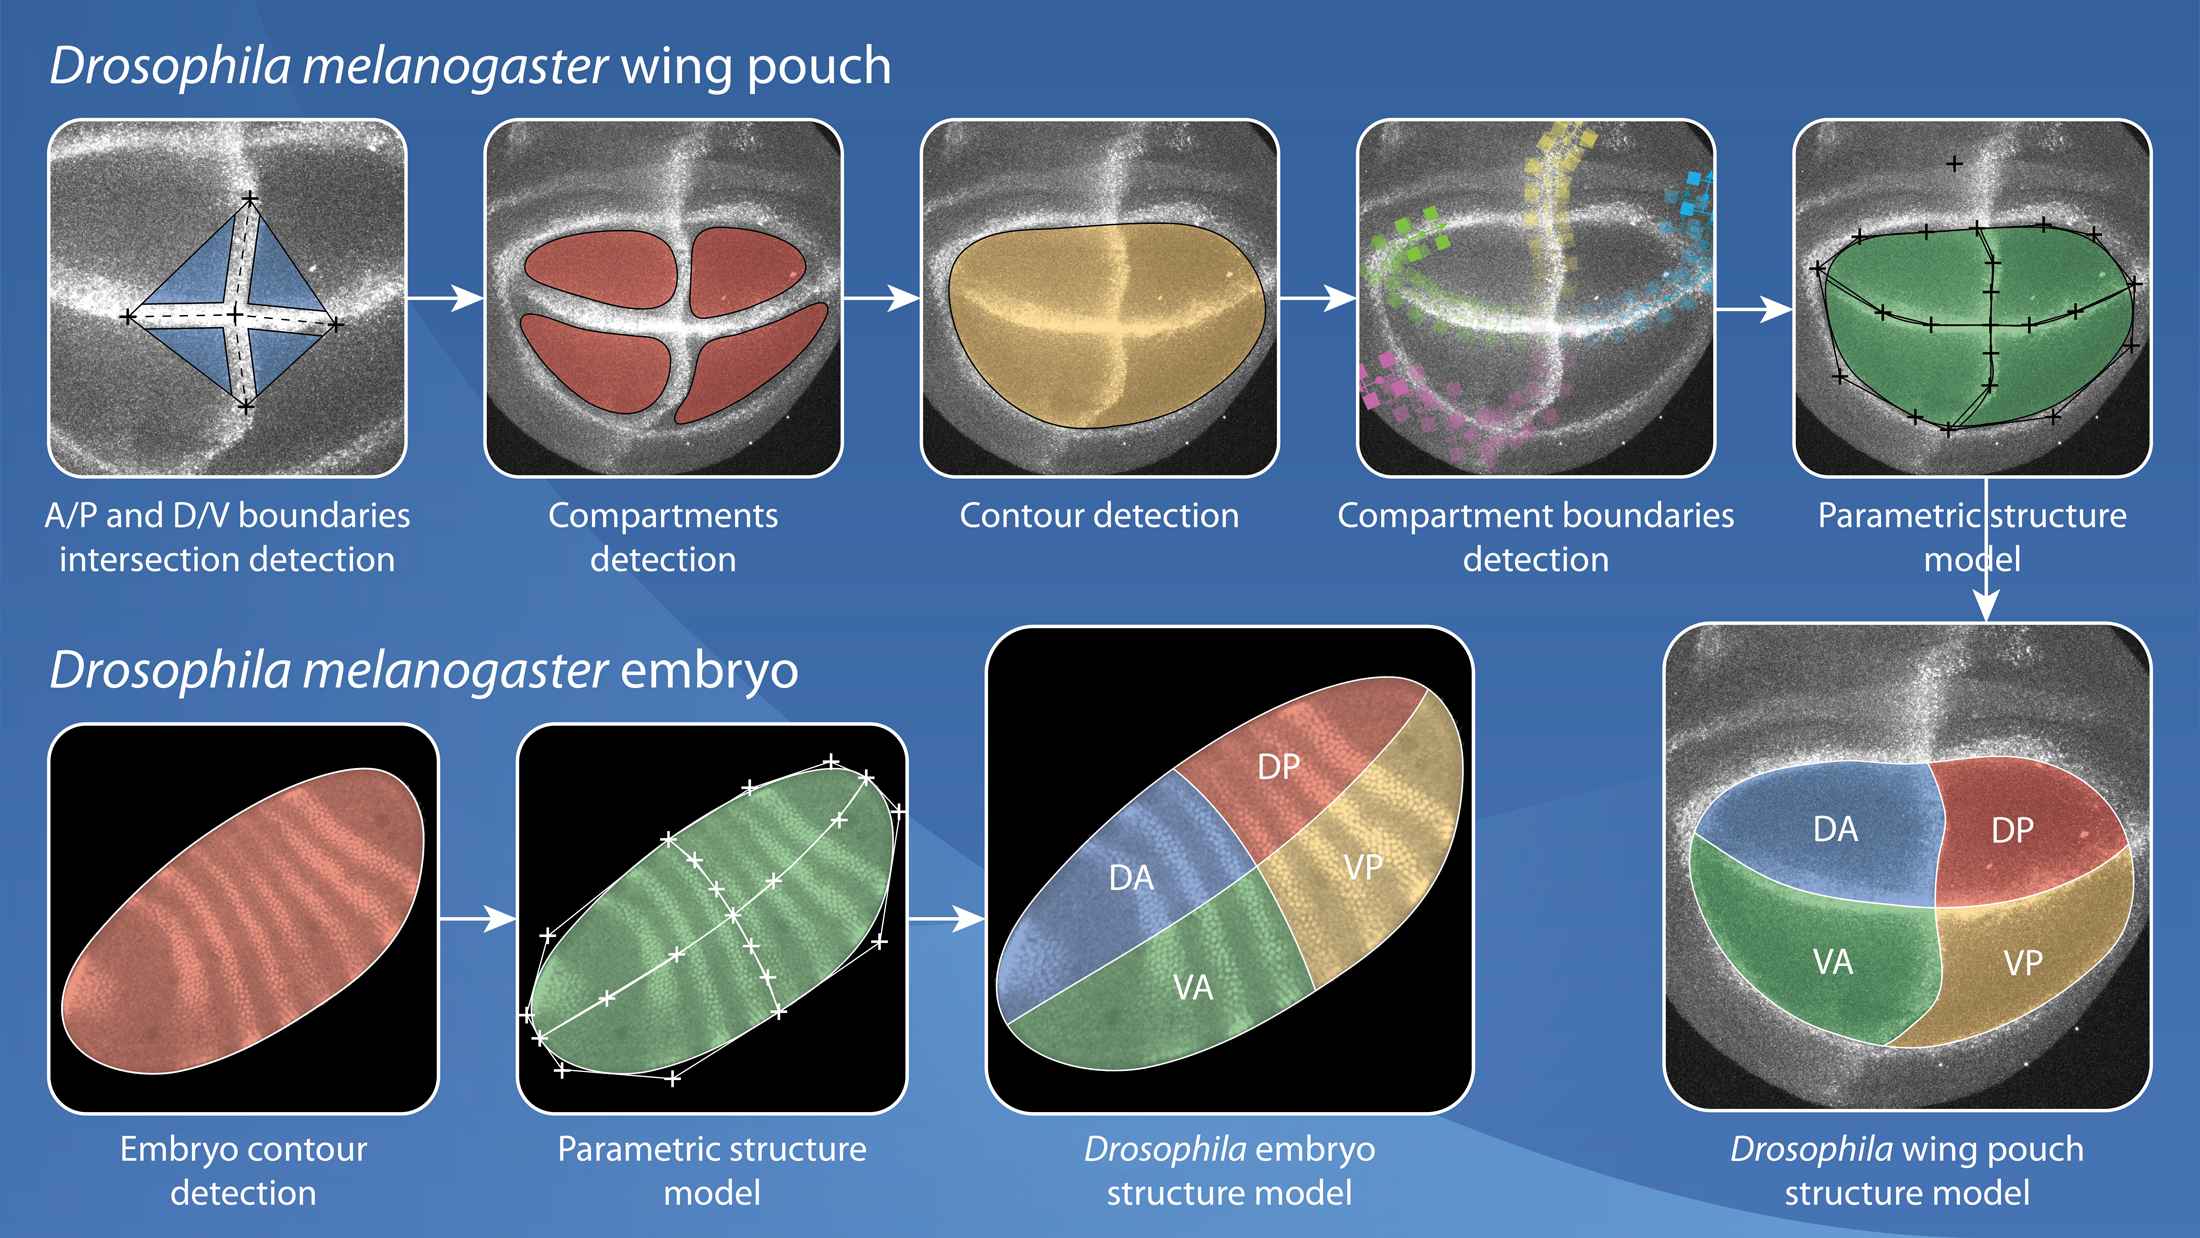
\includegraphics[width=146mm]{images/generic-diagram_300dpi.jpg} % 0.3
\caption{\textbf{Unsupervised inference of a structure models of biological systems from stacks of confocal images.} The structure detection consists in applying many \textit{detection modules} to identify different features of the structure. Here we show the different detection modules we developed to quantify the morphology or structure of the \droso wing pouch and \droso embryo. The outputs of the modules are then integrated to generate a consistent parametric model of the overall structure to describe.}
\label{fig:detection_modules_overview}
\end{figure}

Once a structure model has been inferred, additional tools also available in \wingj to enable the quantification of expression in the space of the structure model. Different approaches are proposed to measure expression including the generation of expression profiles and \textit{expression maps}.\\

Moreover, we developed an automatic 3D cell nuclei detection method to evaluate the number of nuclei in the space defined by the structure model previously inferred using \wingj. This method takes as input a stack of confocal images where nuclei are stained, for instance using nuclear staining such as TO-PRO \autocite{suzuki1997dna} or histone GFP constructs \autocite{kanda1998histone}.\\

% Users can interact with the structure model identified and edit its shape if required by moving around \textit{control points}, which provide a visual representation of the parameters of the model. Finally, the orientation of the structure model (A/P and D/V directions) is automatically inferred based on \textit{a priori} knowledge about the geometry of the wing pouch. Thus, the orientation inference is achieved independently of the orientation of the wing in the XY space of the stack of images.\\


% In \wingj, the structure detection consists in a sequence of \textit{detection modules} designed to identify specific features of the structure to model. For instance in the wing pouch structure detection, one of the first module is applied to identify the point of intersection where the anterior/posterior (A/P) and dorsal/ventral (D/V) boundaries intersect. Later, a second module uses \textit{active contour algorithms} (also called \textit{snakes}) to identify the four compartments DA, DP, VA, and VP that are included in the wing pouch. Then, a parametric model of the structure is generated by combining the output of different modules. We developed as much as eight detection modules to identify the wing pouch structure \citep{schaffter2013}. \wingj allows the user to interact with the parametric model whose shape can be modified by moving \textit{control points}, which are the visual representation of the model parameters. Finally, the orientation (D/V and A/P directions) of the structure model is automatically inferred in \wingj using only prior knowledge about the structure shape for the wing pouch application, for instance. This is achieved so that wings are not required to be perfectly aligned with the borders of the images.\\

In the next sections, we describe how the structure detection from confocal fluorescence images is designed and implemented in \wingj. We also provide guidelines to help developers extending \wingj to quantify the structures of additional organ and body systems. If the guidelines introduced below are followed, the additional tools provided by \wingj for gene expression quantification and nuclei detection, for instance, should be ready to be used with the newly supported systems.

% ===============================================================================
\section{Compiling \wingj}
Download the source code of \wingj from the project web page (\wingjShortUrl). The source code is extensively documented (Javadoc) and the \wingjAPI (Application Programming Interface) is available online.\\

\wingj is released as a Java plugin for \ij (\ijWebsite). Note that \wingj is also supported by \fiji (\fijiWebsite), another distribution of \ij. First, download and install the latest release of \ij. \wingj uses of a few Java libraries that are included in the \textit{lib} folder contained in the ZIP archive of the source code. An Ant script (\textit{build.xml}) is provided to compile \wingj. The script must be edited beforehand to reflect your current setup (e.g. set \ij installation directory). Use the command \textit{ant} where the Ant script is located to build \wingjJar. Then move/copy \wingjJar to the \textit{plugins} folder of \ij before launching \ij. \wingj should now be available in \ij via the menu \textit{Plugins}.\\

For extending \wingj, we recommend to download the source code of \ij and import it in a Java IDE (Integrated development environment) such as \eclipse (\eclipseWebsite). Don't forget to include the Java libraries used by \wingj and \wingjJar itself to the \textit{Java Build Path} of the \ij project. Instead of going through \textit{\ij toolbar $>$ Plugins $>$ \wingj} again and again, the code of \ij can be modified to launch automatically \wingj at \ij startup. One way to do this is to copy/paste the following code at the end of the \emph{main()} method of the \ij class \textit{ImageJ.java}.\\

% \begin{codebox}
\footnotesize\texttt{// ============================================================================\\
// STARTS WINGJ AT IJ STARTUP\\
try \{ \\
\indent \ \ \ WJSettings settings = WJSettings.getInstance();\\
\indent \ \ \ WJPlugIn wingj = new WJPlugIn();\\
\indent \ \ \ wingj.run(null);\\
\indent \ \ \ // WJPlugIn.showAbout();\\
\} catch (Exception e) \{\\
\indent \ \ \ System.out.println("ERROR: Unable to start WingJ from ImageJ.");\\
\indent \ \ \ e.printStackTrace();\\
\}}\normalsize\\
% \end{codebox}

To enable the debug mode in \wingj, set the constant \textit{WJSettings.DEBUG = true} for debugging purpose before compiling \wingj. While coding, use this constant to know when printing debug messages or perform additional tests.

% ===============================================================================
\section{License/How to cite us}
\wingj is released under a \textit{Creative Commons Attribution-NonCommercial-NoDerivs 3.0 Unported License}. A brief description of the license is available at:\\

\href{http://creativecommons.org/licenses/by-nc/3.0/}{http://creativecommons.org/licenses/by-nc/3.0/}\\
% and the full license at\\
% \href{http://creativecommons.org/licenses/by-nc/3.0/legalcode}{http://creativecommons.org/licenses/by-nc/3.0/legalcode}\\

Please cite the papers listed on \wingjUrl when using \wingj in your publications.

% ===============================================================================
\section{How to contact us}
Please feel free to contact the authors with bug reports, feature requests, and information on related projects.

% % \begin{codebox}
% \footnotesize\texttt{Copyright (c) 2010-2012 Thomas Schaffter, Ricard Delgado-Gonzalo\\
% \\
% WingJ is licensed under a\\
% Creative Commons Attribution-NonCommercial-NoDerivs 3.0 Unported License.\\
% \\
% You should have received a copy of the license along with this\\
% work. If not, see http://creativecommons.org/licenses/by-nc-nd/3.0/.\\
% \\
% If this software was useful for your scientific work, please cite our paper(s)\\
% listed on http://lis.epfl.ch/wingj.\\
% \\
% THE SOFTWARE IS PROVIDED "AS IS", WITHOUT WARRANTY OF ANY KIND, EXPRESS OR\\
% IMPLIED, INCLUDING BUT NOT LIMITED TO THE WARRANTIES OF MERCHANTABILITY,\\
% FITNESS FOR A PARTICULAR PURPOSE AND NONINFRINGEMENT. IN NO EVENT SHALL THE\\
% AUTHORS OR COPYRIGHT HOLDERS BE LIABLE FOR ANY CLAIM, DAMAGES OR OTHER\\
% LIABILITY, WHETHER IN AN ACTION OF CONTRACT, TORT OR OTHERWISE, ARISING FROM,\\
% OUT OF OR IN CONNECTION WITH THE SOFTWARE OR THE USE OR OTHER DEALINGS IN\\
% THE SOFTWARE.}\normalsize\\
% % \end{codebox}

